\documentclass[11pt,twoside,a4paper]{article}

\usepackage[utf8]{inputenc} % ajouté
\usepackage[frenchb]{babel}
\usepackage{fourier, erewhon}
\usepackage[T1]{fontenc}
%% permet de spécifier la langue 

\usepackage{indentfirst}
\usepackage{verbatim}
%% pour inclure des figures
\usepackage{graphicx}
%% Pour les maths
\usepackage{amsthm}
\usepackage{amssymb}
\usepackage{amsmath}
\theoremstyle{plain}
\newtheorem{thm}{Théorème}
\newtheorem{prop}{Proposition}
\newtheorem{exo}{Exercice}
\theoremstyle{remark}
\newtheorem{rem}{Remarque}


\parindent 12pt

\pagestyle{plain}


\title{Introduction  {\LaTeX}}
\date{\today}
\author{LABART Céline}
\begin{document}
\maketitle
\section{EXERCICE 1}

\begin{figure}[htbp]
\centering
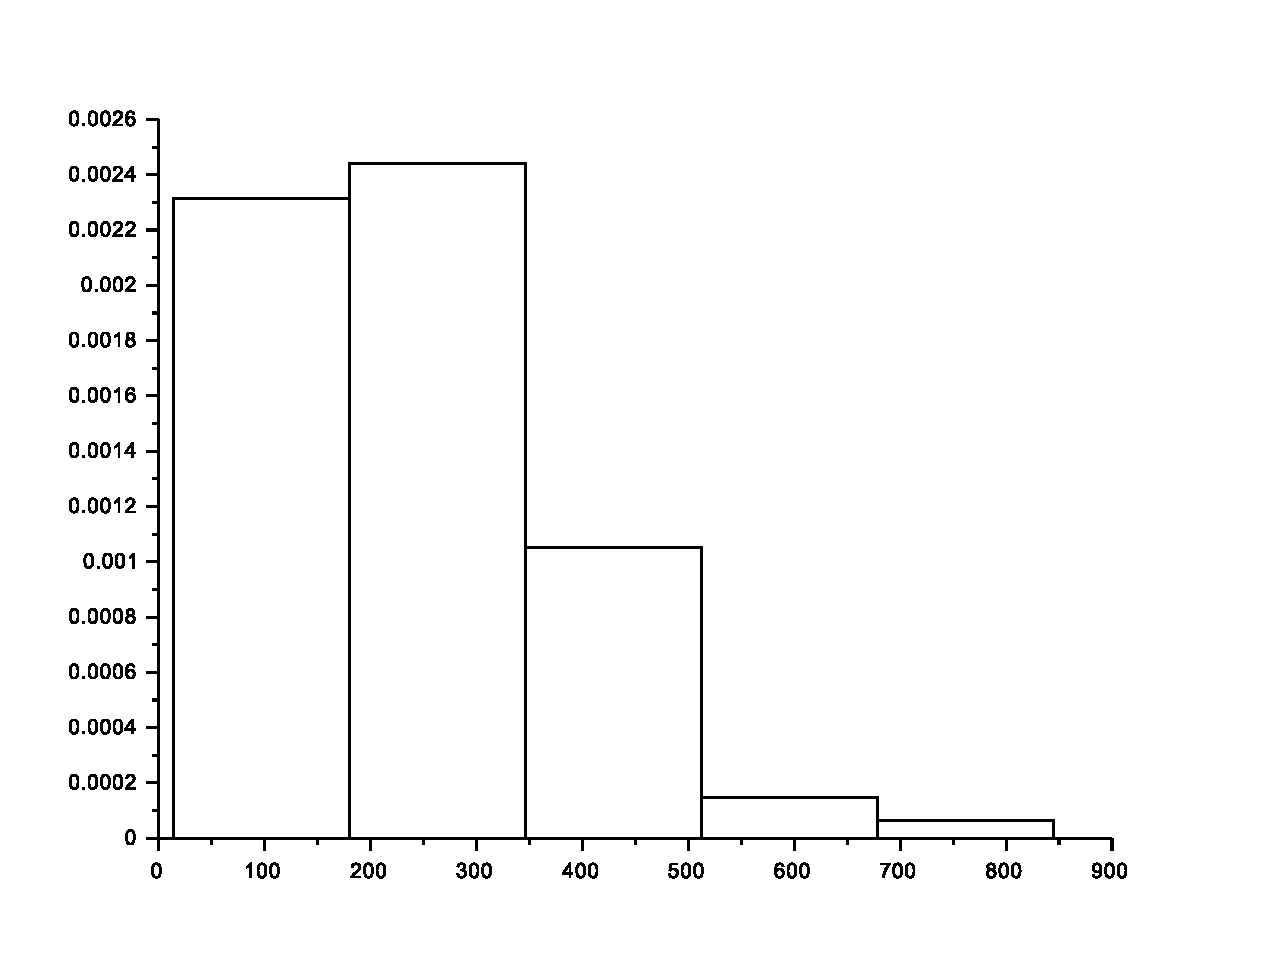
\includegraphics[width=8cm]{hist.pdf}
\caption{graphe de la fonction g sur l'intervalle [1,3]}
\end{figure}

\tableofcontents
\listoffigures

\end{document}
